\section{Numerical approach and results}
\subsection{Numerical implementation}
In order to find Nash equilibria and fix-points of the behaviorally modified Rosenzweig-MacArthur  system \Cref{sec:model_rm}, we use the formulation of \Cref{eq:comp_form}. We discretize space uniformly, using the trapezoidal rule to evaluate the integrals. By using the trapezoidal rule, we keep a banded sparsity pattern in the coupling of the locations. The equations \Cref{eq:dynamics} and the functions $-dU_c, -dU_p$ are formulated via. the symbolic language CasADi \citep{Andersson2019}, where we then solve the complementarity problem as a feasibility problem using IPOPT \citep{wachter2006implementation} using the HSL subroutines for linear algebra \citep{hsl2007collection}. We checked the numerics by also solving the problem with a non-linear complementarity routine from the open-source package SICONOS \citep{acary2019introduction}.

The numerical approach for finding Nash equilibria and fixed points is extremely fast, and should scale to much larger problems. It allows for determination of fixed-points of the dynamics in less than 1 second with several hundred grid points. Simulating the population dynamics is, in contrast, a comparatively slow affair since we simulate the population dynamics using a forward Euler method.

\subsection{Population dynamics}
% on model introduced in \Cref{sec:model_rm}.
With a numerical approach in place, we can study the population dynamics and the sensitivity of \Cref{sec:model_rm} to parameters. We vary the carrying capacity $(K)$ and the intraspecific predator competition $(c)$. We are interested in both  the population levels at equilibrium, and the associated spatial distributions.
The parameters for the model are: \\
\begin{tabular}{l l l}
  Name & Value & Meaning \\
  $K_0$ & $10^{-4}$ & Minimal carrying capacity \\
  $\beta_{p,0}$ & $10^{-4}$ & Minimal predator clearance rate \\
  $\mu_p$ & 0.15 & Predator metabolic rate \\
  $F_p$ & 100 & Predator maximum growth rate \\
  $\epsilon$ & 0.1 & Trophic efficiency
\end{tabular}
\\
\begin{figure}[H]
  \label{fig:pp}
  \caption{Phase portrait of the Rosenzweig-MacArthur system without optimal behavior $(\sigma_c = 1, \sigma_p = 1)$, $(A)$ and with optimal behavior $(B)$ at carrying capacity of $K=40$ and a competition of $c=0$. The green lines show a system trajectory.}
  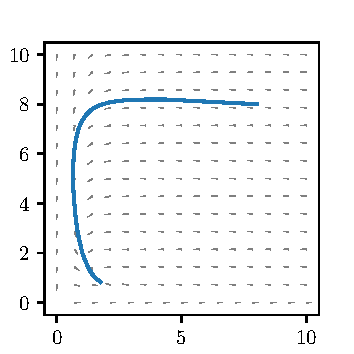
\includegraphics{plots/dynamics.pdf}
\end{figure}
The direction of the flow with optimal behavior (\Cref{fig:pp}(B)) is consistent with the usual Rosenzweig-MacArthur system (\Cref{fig:pp}(A)). The phase portrait reveals that the system dynamics have been stabilized. Looking at the sample trajectory, the system has been overdamped. The stable dynamics stand in contrast to the Rosenzweig-MacArthur model with constant behavior $(\sigma_p=\sigma_c=1)$ where the point of the Hopf bifurcation has been passed \citep{rosenzweig1971paradox}, leading to limit cycles.


\begin{figure}[H]
  \label{fig:dynamic_strategies}
  \caption{Transient strategies of consumers $(A)$ and predators $(B)$ at carrying capacity of $K=40$ and a competition of $c=0$ corresponding to the phase portrait \Cref{fig:pp}.}
  \includegraphics{plots/dynamic_strats.pdf}
\end{figure}
Both consumer and predator strategies change rapidly at the start of the time-interval, before stabilizing towards the equilibrium values. It appears that the consumers are more present in the most productive area when the predator population is lower, which is not that surprising.

\subsection{Population at equilibrium}
\begin{figure}[H]
  \caption{Panel $(A)$ shows population levels of consumers (blue) and predators (red) at equilibrium with changing carrying capacity $(K)$. Panel $(B)$ again shows the population levels, but with varying intraspecific predator competition $(C)$.}
  \label{fig:pop_levels}
  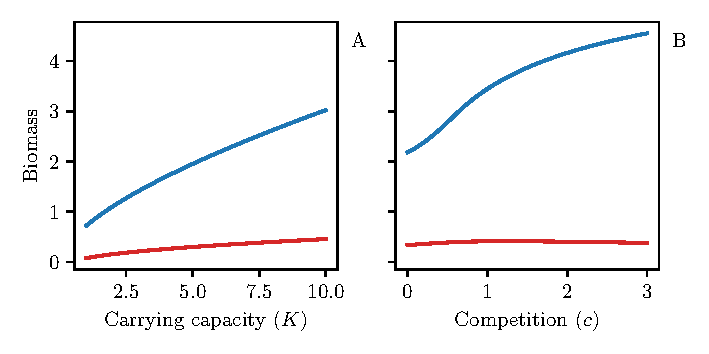
\includegraphics{plots/pop_levels_c.pdf}
\end{figure}
\Cref{fig:pop_levels} reveals how the population levels of consumers and predators change at equilibrium with varying carrying capacity (\Cref{fig:pop_levels}(A)) and intraspecific predator competition (\Cref{fig:pop_levels}(B)).


A higher carrying capacity causes higher populations of both consumers and predators populations at equilibrium (\Cref{fig:pop_levels}). The increase in both populations is probably because the behavioral choice allows the consumers to avoid the risk of predation, while achieving the same fitness.

Varying the intraspecific predator competition causes an increase in the population of predators (\Cref{fig:pop_levels}(C, red)) until a point where the population stabilizes (\Cref{fig:pop_levels}($c\approx 1/3$)). The population of consumers continues to increase (\Cref{fig:pop_levels}(C, blue)) throughout.


\subsection{Spatial distributions}
We start by investigating the spatial distribution of consumers and predators compared to their spatially varying fitness ($-dU_c,~-dU_p$).
\begin{figure}[H]
  \caption{Spatial distribution (full lines) and fitness (dashed lines) of consumers $(A)$  and predators $(B)$ at the equilibrium with carrying capacity $K = 3$.}
  \label{fig:snapshot}
  \includegraphics{plots/snapshot_c.pdf}
\end{figure}
%\Cref{fig:strat_car})
Both consumers and predator distributions have a constant fitness of zero in the area with coexistence, where the fitness of the predators changes when their concentration is zero. In this we recognize the emergence of the ideal free distribution.

\begin{figure}[H]
  \caption{Spatial distribution of consumers $(A)$ and predators $(B)$ at the equilibrium with increasing carrying capacity $(K)$.}
  \label{fig:strat_car}
  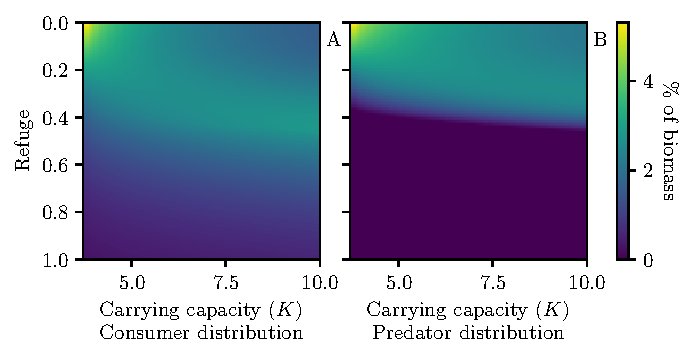
\includegraphics{plots/increasing_car_cap_c.pdf}
\end{figure}
%\Cref{fig:strat_car}) illustrate the strategies of the consumers (\Cref{fig:strat_car}(A)) and predators (\Cref{fig:strat_car}) at equilibrium when carrying capacity varies.

At low carrying capacity consumers are relatively spread out in the most optimal part of the habitat (0-0.3), while predators are concentrated near the most optimal part (0). As the carrying capacity increases, the distribution of consumers becomes more concentrated, distributed around a peak of $0.4$. The peak slowly moves downward with increasing carrying capacity. The consumers can be found throughout the habitat, even at the points of lowest productivity.


Predators go from being concentrated to very spread out, but surprisingly the peak of the predator distribution is just above the peak of the consumer distribution. There are no predators below the band of highly concentrated consumers. This is quite surprising since they have a non-zero encounter rate everywhere. The predator and consumer distributions follow each other as the carrying capacity increases, and appear to approach a stable asymptote.



 %Thus the gain from clustering gradually outweighs the loss from the intraspecific predator competition. That both predator and consumer population increase must be the driving factor behind the peak population concentration moving to less productive areas.

%A higher carrying capacity leads to more concentrated populations, but the increase in populations leads to greater risk-aversion from the consumers so they concentrate in less desirable zones.

\begin{figure}[H]
  \caption{Distribution of consumers $(A)$ and predators $(B)$ at equilibrium under changing predator competition $(c)$.}
  \label{fig:strat_comp}
    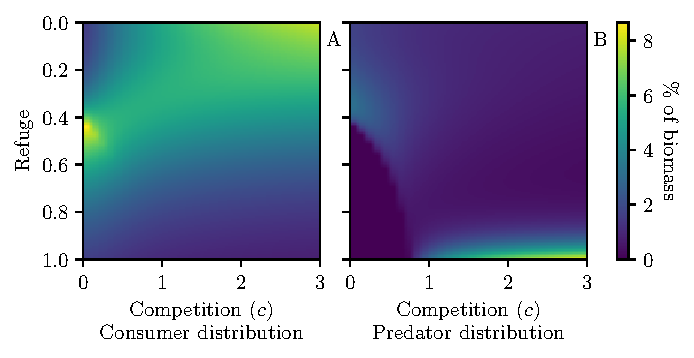
\includegraphics{plots/increasing_competition_c.pdf}
\end{figure}
%In \Cref{fig:strat_comp} the intraspecific predator competition is varied and we see the emergent  equilibrium strategy of the consumers (\Cref{fig:strat_comp}(A)) and predators (\Cref{fig:strat_comp}(B)).

When there is no intraspecific predator competition consumers are highly concentrated at about 0.4, while the predator distributions spreads from 0.4 to 0. The distribution of predators spreads out as we increase competition, before concentrating in the safest zone (1) again. The foraging benefits from clustering on the consumers is outweighed by the risk of encountering other predators. The movement of predators is echoed by the consumers. The consumers spread out and gradually migrate to the most productive area (0). The spreading out of the consumer population though the predator population is concentrated far away is caused by the interspecific competition between consumers, akin to the ideal free distribution. It appears that both consumer and predator densities are converging to asymptotic densities. %An increase in consumer population \Cref{fig:pop_levels} causes an increase in concentration on the less productive spots. When the consumer population spreads out, the distribution trends towards the more productive layers.

\begin{comment}
\begin{figure}[H]
  \caption{Consumer (A) and predator (B) concentration at equilibrium as a function of changing refuge quality}
  \label{fig:ref_qual}

    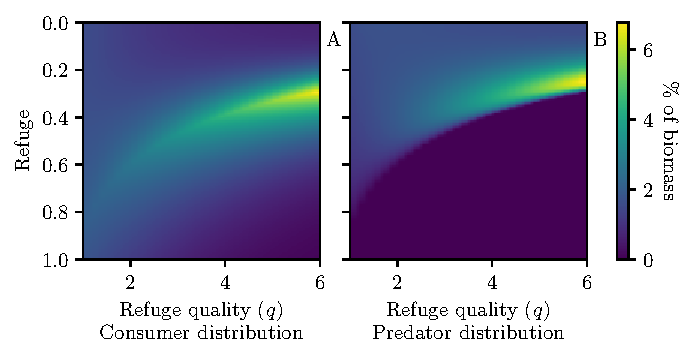
\includegraphics{plots/increasing_refuge_quality_c.pdf}
\end{figure}
\Cref{fig:ref_qual} shows the strategy of consumers (\Cref{fig:ref_qual}(A)) and predators (\Cref{fig:ref_qual}(B)) at equilibrium with varying refuge quality.
\end{comment}
